\documentclass[a4paper,10pt]{article}
%\usepackage[latin1]{inputenc} % Paquetes de idioma (otro encoding)
\usepackage[utf8]{inputenc} % Paquetes de idioma
\usepackage[spanish]{babel} % Paquetes de idioma
\usepackage{graphicx} % Paquete para ingresar gráficos
\usepackage{grffile}
\usepackage{hyperref}
\usepackage{fancybox}
\usepackage{amsmath}
\usepackage{amsfonts}
\usepackage{listings}
% Paquetes de macros de Circuitos
%\usepackage{pstricks}
\usepackage{tikz}

% Encabezado y Pié de página
\usepackage{fancyhdr} % Paquete para encabezados y pie de página
\pagestyle{fancy} % Sin esta línea no se imprimiría el encabezado en todas las páginas

\fancyhf{} %  Borra el encabezado anterior (Por defecto escribe el títutlo de la sección en la que se encuentra la hoja
\setlength{\headheight}{22.55pt}
\fancyhead[L]{
	{\textsf{Facultad de Ingenier\'ia $-$ Universidad de Buenos Aires \\ 66.09 Laboratorio de Microcomputadoras}}
}
%\addtocounter{page}{5}
\fancyhead[R]{\thepage}

\renewcommand{\footrulewidth}{0.4pt} % Ajusta el tamaño de las líneas separadoras en el pié de página
\renewcommand{\headrulewidth}{0.4pt} % Ajusta el tamaño de las líneas separadoras en el encabezado

\fancyfoot[L]{
	{\textsf{Anteproyecto} \\
	{\textsf{Integrantes: Torres Feyuk, Levi Hadid}}
	}
}
		

% Carátula del Trabajo
\title{ \author{} % Lo pongo para que el warning no moleste :p
\setlength{\unitlength}{1cm} %  Especifica la unidad de trabajo
\thispagestyle{empty}

\begin{picture}(18,0)
\put(0,0){
\includegraphics[width=1.5cm, height=3cm]{Imagenes/Logo1.png}}

\put(10.5,0){
\includegraphics[width=3cm, height=3cm]{Imagenes/Logo2.png}}

\end{picture}
\\[1.5cm]
\begin{center}
	\textbf{{\Huge Facultad de Ingenier\'ia \\ Universidad de Buenos Aires}}\\[2cm]
	{66.09 Laboratorio de Microcomputadoras}\\[0.5cm]
	{Anteproyecto}\\[2.5cm]
\end{center}

\begin{flushleft}
	\textbf{Integrantes:} \\[1cm]

	\begin{tabular}{|c|c|c|}
		\hline
		\textbf{\normalsize Padr\'on} & \textbf{\normalsize Nombre} & \textbf{\normalsize Email} \\
		\hline
		\normalsize 89579 & \normalsize Torres Feyuk, Nicol\'as R. Ezequiel & \normalsize ezequiel.torresfeyuk@gmail.com \\
		\hline
		\normalsize 90406 & \normalsize Levi Hadid, Lucas Alberto & \normalsize lucaslh9@hotmail.com \\
%		\hline
%		\normalsize ????? & \normalsize Madariaga, Eduardo & \normalsize madariagaedu@gmail.com \\
		\hline
	\end{tabular}
\end{flushleft}
\date{} % Hace que no se imprima la fecha en la cual se compilo el .tex
 }

\begin{document}
	\maketitle % Hace que el título anterior sea el principal del documento
	\newpage

	\tableofcontents % Esta línea genera un indice a partir de las secciones y subsecciones creadas en el documento
	\newpage

	\section{Proyecto: Autito RC}
		El proyecto a realizar es un autito manejado a través de comunicación inalámbrica por un medio control remoto (estos autos son los llamados \emph{RC cars}).
		Las tarea a desarrollar por el grupo consiste en diseñar el circuito de control que permita manejar el autito. Para esta tarea se utilizarán dos
		microcontroladores de la familia Atmel, uno para el circuito del auto y el otro para el circuito del control remoto. \\
		\indent Además de la función básica de poder manejar al autito a través del control, se le agregarán al mismo algunas funcionalidades de forma de 
		poder explotar la potencia y flexibilidad de los microcontroladores. \\
		\indent Cabe destacar que la parte mecánica del auto no será diseñada por los integrantes del grupo, sino que se utilizará un miniauto el cual ya viene 
		con la parte mecánica desarrollada.

	\section{Miniauto}
		El autito conseguido para implementar la parte del control es un vehículo con tracción delantera. El mismo posee un motor de continua para mover las
		ruedas traseras y un servo para girar las ruedas delanteras. Dadas las funcionalidades que desean agregarse, la carcaza tanto del
		control remoto como del auto seguramente no serán  utilizadas, pero al menos se intentará mantener el chasis del vehículo para no modificar la
		parte mecánica del mismo.	

	\section{Funcionalidades}
		A continuación se describen las funciones que serán desarrolladas tanto para el autito como para el control remoto:
		\subsection{Autito}
			\subsubsection{Control de Motores}
				La parte mecánica del miniauto consiste en controlar el tanto el servo como el motor de continua. Para desarrollar esta tarea, se utilizarán dos
				puentes H (uno para cada motor), de modo de poder controlar tanto la velocidad del vehículo como el sentido de giro.  
			\subsubsection{Bumpers (Parachoques)}
				En la parte delantera del auto se colocarán dos bumpers. Un bumper es un conmutador de 2 posiciones con muelle de retorno a la posición de reposo
				y con una palanca de accionamiento. Mediante este dispositivo se detectarán choques en la parte frontal del auto. Al chocar el auto, se deberá
				enviar al control remoto una señal avisando de este evento. 
			\subsubsection{Emisor - Receptor (Puerto Serie)}
				La comunicación con el control se realizará a través del puerto serie disponible por los microcontroladores utilizados. La comunicación inalámbrica
				se realizará a través de del protocolo ZigBee u otro protocolo. En el caso de la comunicación inalámbrica por ZigBee, el LABI nos provee los 
				integrados que nos permite convertir la comunicación serial a inalámbrica, de forma que en una primera instancia se pensará a la misma como si fuera
				serial y no remota.
			\subsubsection{Diagrama En Bloques}
				\begin{figure}[!htb]
						%\centering
						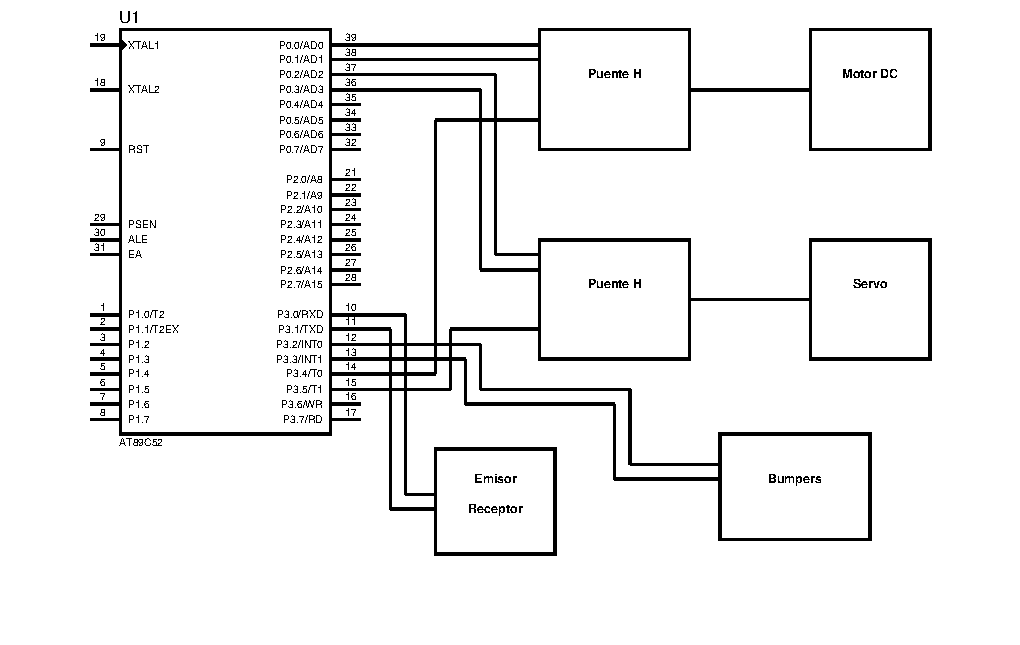
\includegraphics[width=13cm]{Imagenes/DiagramaAutito.pdf}
						\caption{Diagrama en Bloques del Autito} \label{img001}
					\end{figure}
				
		\subsection{Control Remoto}
			\subsubsection{Velocidades (Caja de Cambios)}
				A partir de un par de botones, se podrá ir variando la velocidad del miniauto. La cantidad de velocidades que poseerá el mismo aún no está definido.
				El control poseerá un botón para aumentar la velocidad y otro para decrementar la velocidad.
			\subsubsection{Display Indicador Velocidad}
				Para poder indicar la velocidad actual del auto, se incluirá en el control un display de 7 segmentos. La decodificación entre la palabra a mostrar
				por el 7 segmentos y el número en cuestión en un principio será realizada por el microcontrolador. 
			\subsubsection{Motor Vibrador}
				Se incluirá en el control un motor vibrador. El mismo vibrará cada vez que el autito choque frontalmente contra algún objeto, activando los bumpers
				del mismo. 
			\subsubsection{Emisor - Receptor (Puerto Serie)}
				La comunicación entre el autito y el control se realizará de la misma forma en los dos circuitos, de la forma explicada en la sección del auto.
			\subsubsection{Diagrama En Bloques}
				\begin{figure}[!htb]
						\centering
						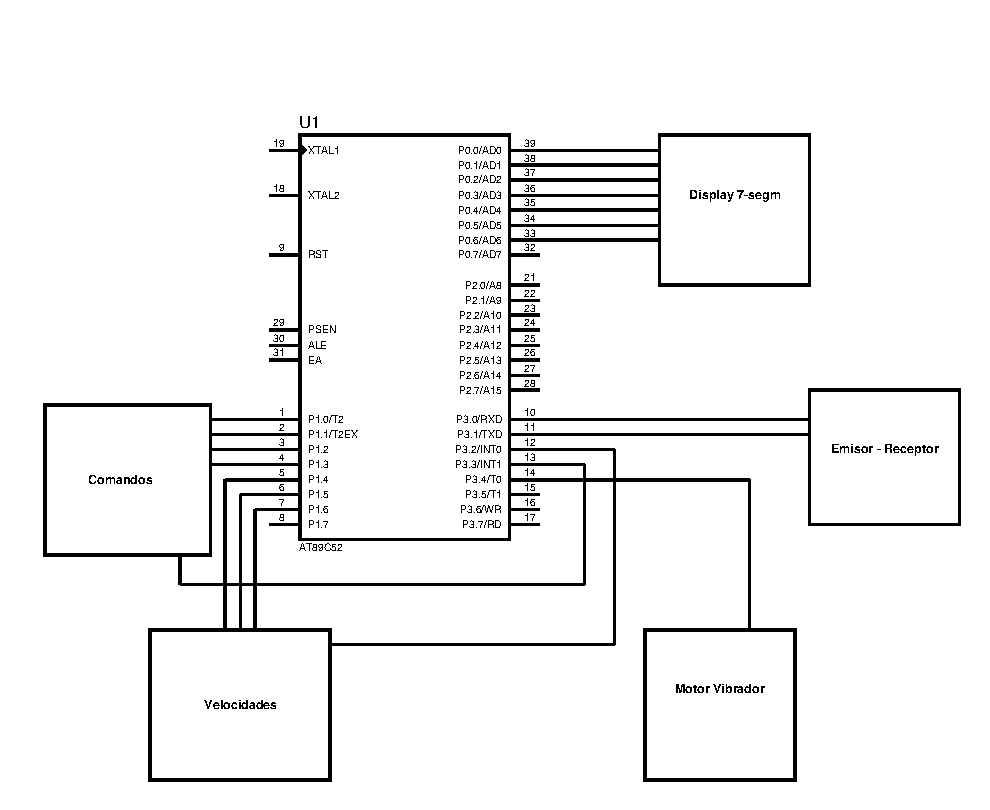
\includegraphics[width=13cm]{Imagenes/DiagramaControl.pdf}
						\caption{Diagrama en Bloques del Control Remoto} \label{img002}
					\end{figure}
	
		\section{Software}
			Tanto el control como el autito 
			\subsection{Diagrama de Flujo (Comunicación Serie - Motores)}
				\begin{figure}[!htb]
						\centering
						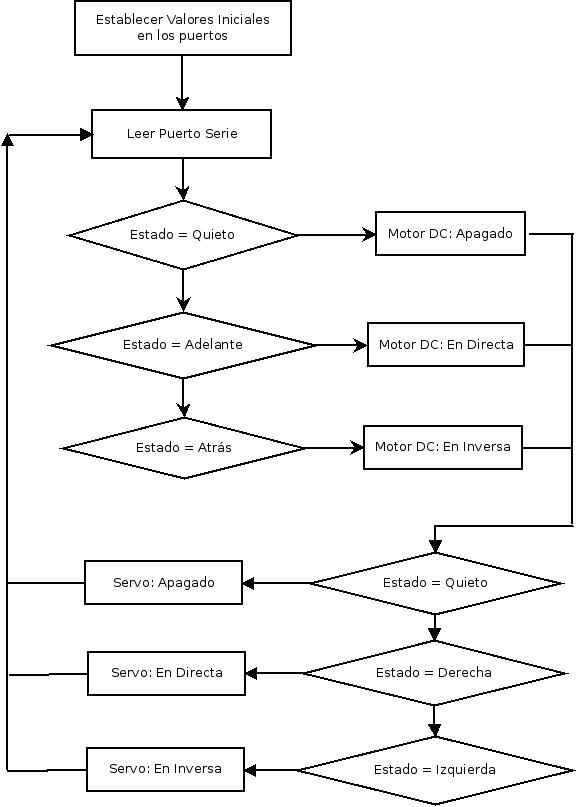
\includegraphics[width=11cm]{Imagenes/DiagramaFlujoAutito.jpeg}
						\caption{Diagrama en Bloques del Control Remoto} \label{img003}
					\end{figure}
\end{document}
